\section{Kanalcodierung}
\subsection{Bitfehlerwahrscheinlichkeit $\varepsilon$}
$\varepsilon$ ist die Wahrscheinlichkeit, dass ein Bitfehler auftritt (BER - Bit Error Rate).
\begin{itemize}
	\item Alle Bits falsch: $BER = 1$
	\item Kein Bit falsch: $BER = 0$
	\item 1 von 2 Bits falsch: $BER = 0.5$
	\item 1 von 1000 Bits falsch: $BER = 0.001$
\end{itemize}
\subsection{Binary Symmetric Channel (BSC)}
Bei $x_1$ und $x_0$ kommen jeweils 0 oder 1 hinen. Die Wahrscheinlichkeit, dass ein Bitfehler auftritt, ist $\varepsilon$.
Die Wahrscheinlichkeit dass kein Bitfehler auftritt, ist $1 - \varepsilon$.
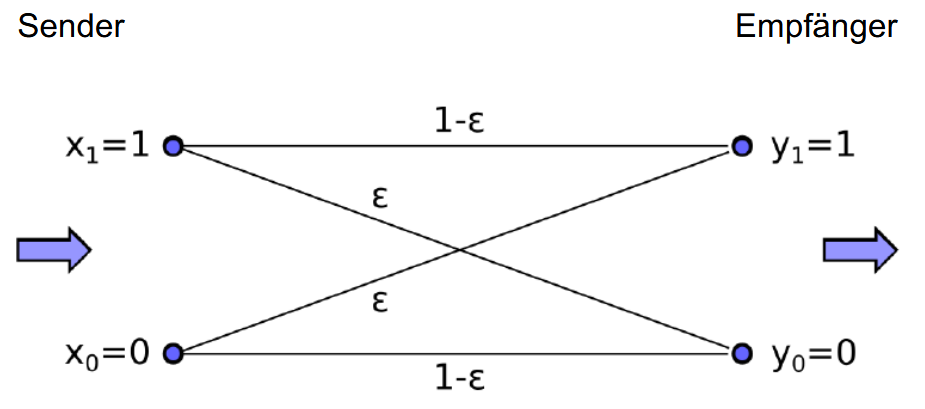
\includegraphics[scale=0.4]{bsc}
\subsubsection{Erfolgswahrscheinlichkeit}
\begin{align*}
	P_{0,N} = \frac{A_N}{A} = (1 - \varepsilon)^N
\end{align*}
\subsubsection{Fehlerwahrscheinlichkeit}
Auf $N$ Datenbits:
\begin{align*}
	1 - P_{0,N} = 1 - (1 - \varepsilon)^N
\end{align*}
Wobei für $N \cdot \varepsilon \ll 1$ folgende Näherung gilt: $1 - (1 - \varepsilon)^N \approx ( 1 - N \cdot \varepsilon)$
\subsubsection{Mehr-Bit-Fehlerwahrscheinlichkeit}
\begin{itemize}
	\item $\binom{N}{F}$: Anzahl der Möglichkeiten, $F$ Fehler in $N$ Bits zu platzieren.
	\item $\varepsilon^F$: Wahrscheinlichkeit, dass $F$ Fehler auftreten.
	\item $(1 - \varepsilon)^{N-F}$: Wahrscheinlichkeit, dass Alle restlichen Bits $N-F$keinen Fehler haben.
\end{itemize}
\begin{align*}
	P_{F,N} = \binom{N}{F} \cdot \varepsilon^F \cdot (1 - \varepsilon)^{N-F}
\end{align*}
$\binom{N}{F} = \frac{N!}{F! \cdot (N-K)!}$ bzw. $\binom{6}{2}$ rechnet man wie folgt:
\begin{align*}
	\binom{6}{2} = \frac{6!}{2! \cdot (6-2)!} = \frac{6 \cdot 5 \cdot 4 \cdot 3 \cdot 2 \cdot 1}{2 \cdot 1 \cdot (4 \cdot 3 \cdot 2 \cdot 1)}
	= \frac{6 \cdot 5 \cdot \cancel{4 \cdot 3 \cdot 2 \cdot 1}}{2 \cdot 1 \cdot \cancel{(4 \cdot 3 \cdot 2 \cdot 1)}}  = \frac{6 \cdot 5}{2 \cdot 1} = 15
\end{align*}
\subsubsection{Coderate $R$}
\begin{itemize}
	\item Die Coderate $R$ ist das Verhältnis von Nutzdatenbits zu gesendeten Bits.
	\item $K$ ist die Anzahl der Nutzdatenbits und $N$ die Anzahl der gesendeten Bits.
	\item Z.B. $Paritaetsbits + Informationsbits = N$\\ und $K = Informationsbits$.
\end{itemize}
\begin{align*}
	R = \frac{K}{N}
\end{align*}
\subsubsection{Kanalkapazität $C$}
Die Kanalkapazität $C$ in $bit/bit$ ist die maximale Datenrate, die über einen Kanal übertragen werden kann.
\begin{align*}
	C_{BSC}(\varepsilon) = 1 - H_b(\varepsilon)
\end{align*}
\subsubsection{Kanalkodierungstheorem}
Möchte man die Restfehlerwahrscheinlichkeit eines Fehlerschutzcodes beliebig klein machen,
so muss $R < C$ sein.
\subsection{Hamming-Distanz}
Die Hamming-Distanz $d_H$ ist die Anzahl der unterschiedlichen Bits zwischen zwei Codewörtern.\\
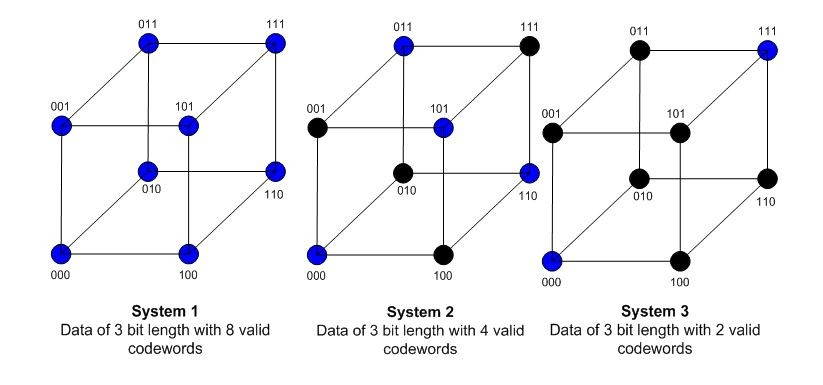
\includegraphics[scale=0.45]{hamming}
\subsubsection{Eigenschaften}
\begin{itemize}
	\item \textbf{Systematisch}: Ein Code ist Systematisch wenn die Nutzdatenbits unverändert im Codewort übernommen werden.
	      Hierfür müssen legendlich z.B. die Paritätsbits entfernt werden.
	\item \textbf{Linear}: Ein Code ist linear wenn jede Kombination ($EXOR$) von Codewörtern wieder ein Codewort ist.
	\item \textbf{Zyklisch}: Ein zyklischer Code ist eine spezielle Art eines linearen Codes, bei dem jede
	      zyklische Verschiebung eines Codeworts ebenfalls ein gültiges Codewort ist.
	\item \textbf{Perfekt}: Ein Code heisst ein «perfekter Code», wenn jedes empfangene Wort $w$
	      genau ein Codewort $c$ hat, zu dem es eine geringste Hamming-Distanz
	      hat und zu dem es eindeutig zugeordnet werden kann.
\end{itemize}
\subsection{Paritätscheck}
\subsubsection{1D Paritätscheck}
Ein Parity-Bit bestimmt, ob die Anzahl Einer in einem Codewort gerade oder ungerade ist.
Even und Odd Parity sind gleichwertig, wobei nur even parity lineare Codes ermöglicht.
\subsubsection{2D Paritätscheck}
Ein 2D Paritätscheck...
\begin{itemize}
	\item ...ist ein Paritätscheck, der auf zwei Dimensionen angewendet wird.
	\item ...kann einen Fehler in einer Zeile oder Spalte erkennen und korrigieren.
	\item ...kann zwei Fehler erkennen, aber nicht korrigieren.
	\item ...kann drei Fehler nicht erkennen.
\end{itemize}
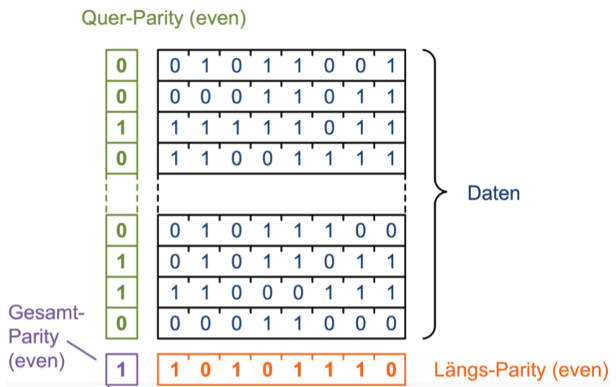
\includegraphics[scale=0.5]{2d_parity}

\subsection{CRC}
\subsubsection{CRC-Polynomdivision}
\begin{itemize}
	\item Nutzdatenwort: $111010100$
	\item Generatorpolynom: $x^3 + x^2 + 1 \Rightarrow$ $\textcolor{blue}{1101}$
	\item Nutzdatenwort mit Nullen (Grad des Generatorpolynoms [3]) erweitern: $111010100\textcolor{red}{000}$
	\item Rest bestimmen durch Division: $100$
	\item Rest an Nutzdatenwort anhängen: $111010100\textcolor{red}{100}$
\end{itemize}
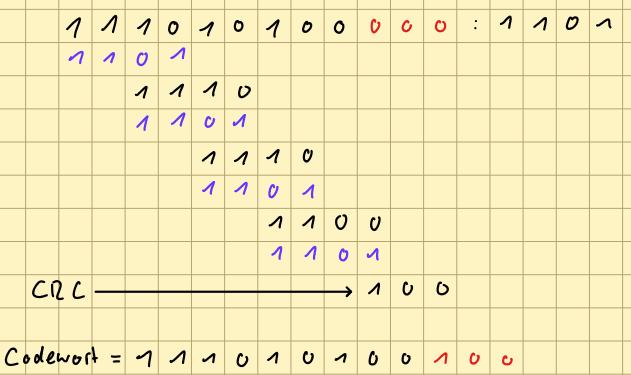
\includegraphics[scale=0.55]{crc_div}
\subsection{Blockcodes}
Lineare Blockcodes werden über eine Generatormatrix
definiert. Das Codewort entsteht indem die Daten mit der
Generatormatrix multipliziert werden:\\
\begin{align*}
    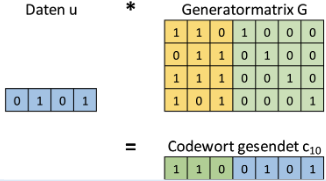
\includegraphics[scale=1]{blockcode1}
\end{align*}
\subsubsection{Bildung Generatormatrix}
\begin{align*}
    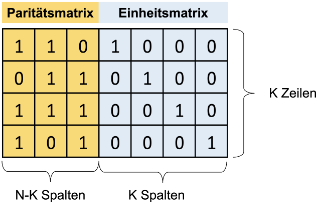
\includegraphics[scale=0.8]{blockcode2}
\end{align*}
Die Paritaetsbits (Zeilen) müssen voneinander linear unabhängig sein.
Für Hamming-Codes gilt: Jede Zeile hat gleich viele Einsen wie $d_{min}$.
\begin{align*}
    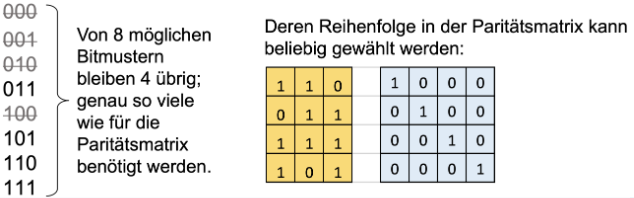
\includegraphics[scale=0.6]{blockcode3}
\end{align*}
\subsubsection{Bildung Prüfmatrix}
\begin{align*}
    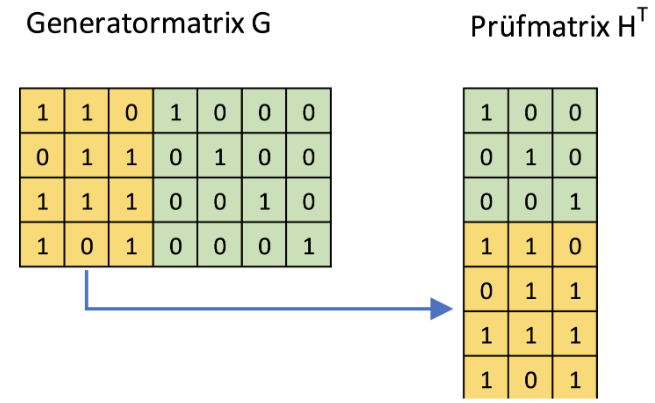
\includegraphics[scale=0.5]{blockcode4}
\end{align*}
\begin{align*}
    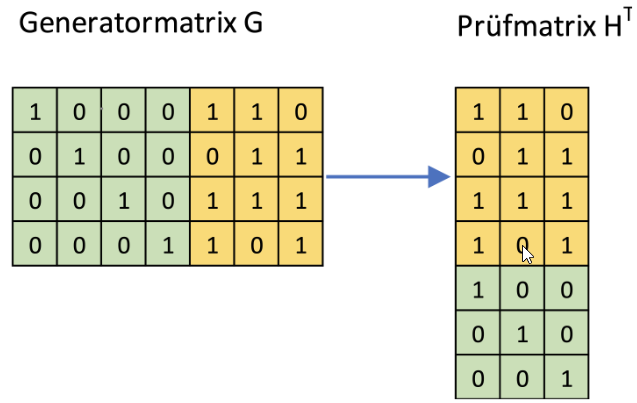
\includegraphics[scale=0.5]{blockcode5}
\end{align*}

\subsection{Faltungscodes}
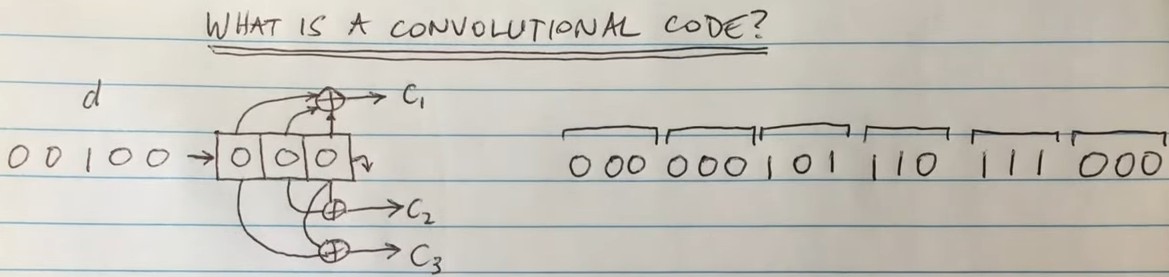
\includegraphics[scale=0.31]{faltungscode}
\subsubsection{Trellis Diagramm}